\chapter{File Protection}
	\section{Built in protection}
	\paragraph{}
	Usually, operating systems do not have a built in mechanism that include a password protection method. However, there is a file permission policy that counts as a level of protection from other users.
	
	\subsection{Windows}
	\paragraph{}
	File protection in Windows can be achieved through DACLs (discretionary access control lists). As a short explanation, a Windows object can have a DACL which contains ACEs(access control entries) that define what type of access any user or group of users can have\cite{MDSNDACsLACEs}.
	
	\paragraph{}
	Usually, DACLs are used by defining the users and groups that can have access because the ones that are not included will have restricted access by default. If a DACL does not contain any ACEs the system will deny any type of access.
	
	\begin{figure}[h!]
		\includegraphics[width=\linewidth]{images/securitySettings.jpg}
		\caption{Advanced Security Settings dialog}
		\label{fig:securitySettings}
	\end{figure}
	
	\paragraph{}
	Let us consider a new text file named "demo file.txt" on a Windows 10 OS that has 2 users, namely user and user 1, which both have administrator permissions. To restrict access for user 1 I have to go to file's properties \textbf{Security}-\textgreater\textbf{Advanced}.
	
	\paragraph{}
	In figure \ref{fig:securitySettings} we can see the "Permission Entries" which maps to DACL we mentioned earlier whilst list's entries map to ACEs. I added the Administrators group and user to have full control, and also I set user 1's permissions to deny any type of action. In this example we can notice that the order in which permissions are set matters because user 1 cannot access the file, even if that user takes part from Administrator's group. 
	
	\paragraph{}
	At the moment only the current user and other possible users in the Administrator group could have access to the file. Still, we are not fully protected when it comes for example to exploits. We could consider that we are logged in with user 1, which currently does not have any kind of permission for the demo file. There is the possibility of an exploit having first user's permissions and overwriting, encrypting or deleting the file which would be disastrous.
	
	\subsection{Linux}
	\paragraph{}
	A similar mechanism exists in Linux, but it's more trivial. In my examples I will talk about Ubuntu, but the matter is almost the same for most of the Linux distributions.
	
	\paragraph{}
	For every file in Linux we have permissions for three main user groups: owner of the file, owner's group and all other users. 
	
	\begin{figure}[h!]
		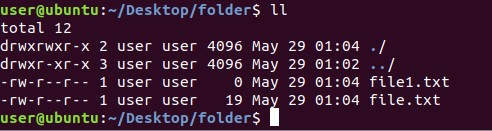
\includegraphics[width=\linewidth]{images/linuxFilePermissions.jpg}
		\caption{Linux file permissions}
		\label{fig:linuxFilePermissions}
	\end{figure}
	
	\paragraph{}
	Figure \ref{fig:linuxFilePermissions} displays in the first column 10 characters, 9 of which represent the permissions for every file and directory. The first character represents the type of item, which can be a file or a directory. The next characters are split in sets of three: the first set represents user's permission, the middle set is for group permissions, and the last set represents the permissions for other users. For the described three-character groups we can have the following possible values:
	\begin{itemize}
		\item "-" - restricted access
		\item "r" - read permission
		\item "w" - write permission
		\item "x" - execute permission
	\end{itemize}
	
	\paragraph{}
	The ownership of a file can be changed through chown command whilst the permissions of the file can be changed with chmod command, so the user can decide if the file can be accessed by others. This approach is more generic than the Windows mechanism because you cannot specify the rights for every user or group of users.
	
		
	\section{Existing products for Windows}
	\paragraph{}
	As a similar tool, a first one that draws attention, is iBoysoft's File Protector for Windows, coming as a 7-day free trial or a payed version. As a main functionality, this tool allows the user to select the desired folders or files to be protected, along with the protection type which can be:
	\begin{itemize}
		\item read
		\item write
		\item delete
	\end{itemize}
	
	\paragraph{}
	The application starts with a message box, demanding a password. After it was inserted correctly, the main screen is displayed, containing a list of files and folders the user has chosen to be protected along with the protection type for each one of them.
	
	\begin{figure}[h!]
		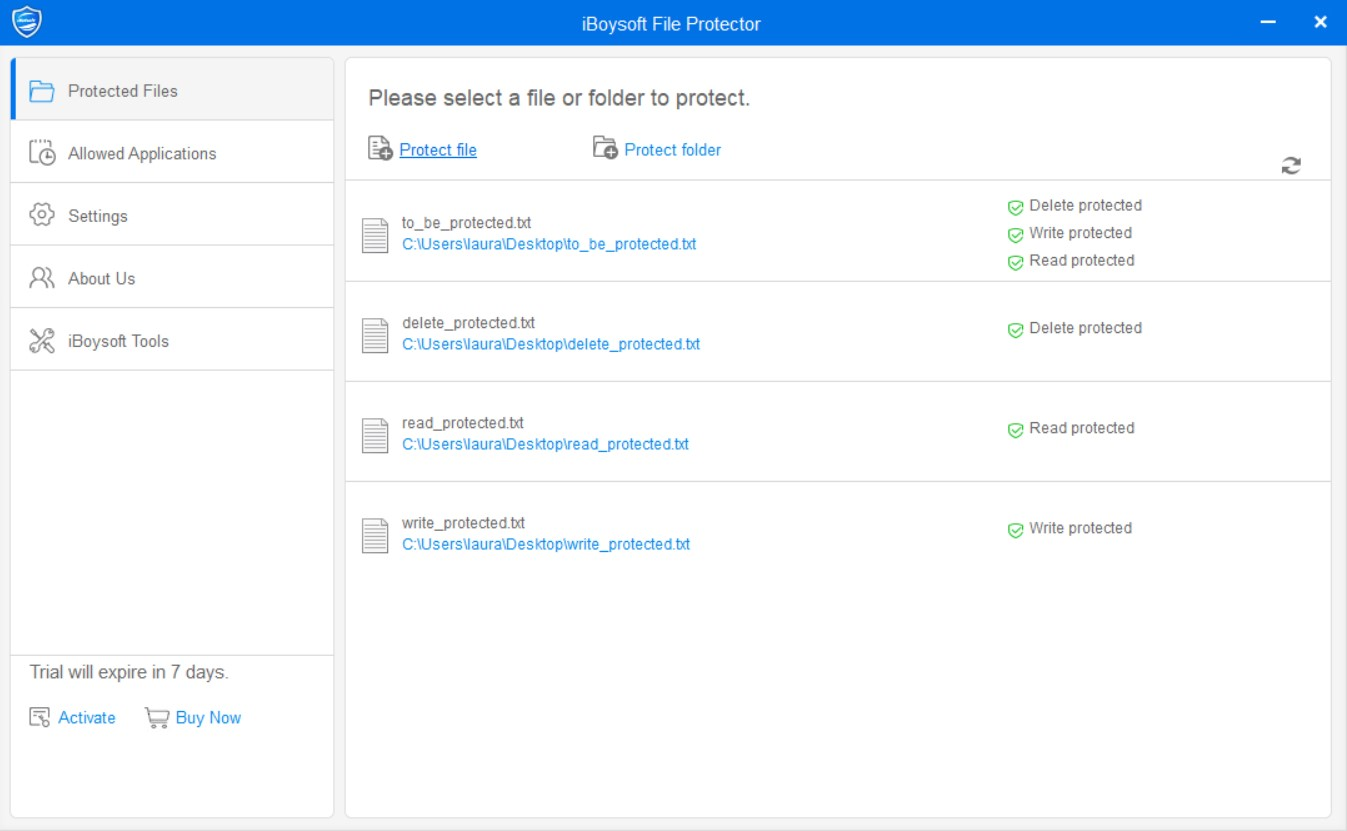
\includegraphics[width=\linewidth]{images/iBoysoftMain.jpg}
		\caption{iBoysoft File Protector for Windows}
		\label{fig:iBoysoftFP}
	\end{figure}
	
	\paragraph{}
	In figure \ref{fig:iBoysoftFP} we can see the main screen of the application, where we have a list of protected files, buttons for adding files or folders, and also the menu on the left. 
	
	\paragraph{}
	Another feature of this tool can be found in the "Allowed Applications" tab. There, the user can choose a set of applications which can access the protected items, in spite of the protection selected for them. However, adding an application demands also selecting the files which can be manipulated by it.
	
	\paragraph{}
	There is also the settings tab which contains two sections, one where you can change the password request at application's startup, and another one where you can choose the default protection types that are selected when adding a file or folder. The second feature is a useful one because the user can select a default way for files to be protected when they are added into the list, skipping a set of settings to be made for every file addition.
	
	\paragraph{}
	An example of a drawback of this application would be adding a text file for reading protection because the user cannot access it afterwords using any kind of application. However, the user can give permissions to other applications to perform actions upon the desired files. This way a user can access the file just by using that exact set of applications.
	
	\paragraph{}
	As a conclusion, this application provides security for a set of files which the user has selected as being protected. Moreover, there are a set of applications that a user can select to have permissions over desired files. However, the only time a password is required, is when the application is started. 
	
	\newpage
	\section{Linux Implementation Overview}
	\paragraph{}
	This section is focused on presenting a potential implementation for the file protector filter on UNIX systems. There are two theoretically possible approaches. The first one leverages the VFS in implementing a "Filter Manager"-like framework. The second one is a more intrusive and dangerous technique that is based on system call hooking. 
	
	\subsection{RedirFS}
	\paragraph{}
	As stated in the RedirFS paper, it is a new layer between VFS (virtual file system switch) and file system drivers\cite{RedirFS}. It is implemented as a standalone kernel module and modifies file system calls in VFS in order to provide a minfilter-like experience for filtering file system operations.
	
	\paragraph{}
	The Virtual File System (also known as the Virtual Filesystem Switch) is the software layer in the kernel that provides the filesystem interface to userspace programs. It also provides an abstraction
	within the kernel which allows different filesystem implementations to coexist\cite{KernelArchivesVFS}. This mechanism is very similar to the Windows I/O System which will be detailed later in this chapter.
	
	\paragraph{}
	The VFS is the glue that enables system calls such as \texttt{open()}, \texttt{read()}, and \texttt{write()} to work regardless of the filesystem or underlying physical medium\cite{LinuxKernelDevelopment}. VFS provides an interface that is implemented by file system drivers, such as Ext4. The file concept is the base of VFS, because everything is viewed as a file. ProcFS is an example of a pseudo-file system driver, because it uses the VFS to expose a file system-like interface to the user. In instance, a user could query the running processes list either by the traditional \texttt{ps} command or, by making use of VFS, a user could use \texttt{ls} command to list processed in the following manner:
	
	\paragraph{}
	\bigskip
	\centerline{ls $-$l /proc}
	\bigskip
	
	This command will show us the active processes by showing a directory for each process, with the process PID as the directory name. This also shows other relevant system information, such as PCI connected devices (/proc/bus/pci).
	
	\paragraph{}
	VFS uses 4 type of objects, namely:
	
	\begin{itemize}
		\item superblock object, which represents a specific mounted system
		\item inode represents a file 
		\item dentry is a directory entry which represents a single component of a path
		\item file object represents an opened file
	\end{itemize}
	
	Each of the aforementioned contains an operations object which are pointers to functions that the kernel invokes against the primary objects.
	
	\paragraph{}
	The file\_operations structure contains two function pointers that are of interest in the context of implementing a file protector on Linux: \\
	
	\begin{Verbatim}[fontsize=\small, commandchars=\\\{\}]
	struct file_operations \{ 
		...
		int (*open) (struct inode *, struct file *); 
		...
		int (*release) (struct inode *, struct file *); 
		...
	\}	
	\end{Verbatim}
	
	The \texttt{open()} callback creates a new file object and links it to the corresponding inode object. It is called by the \texttt{open()} system call\cite{LinuxKernelDevelopment}. This is the most important callback because it allows synchronous interception of file open semantics as well as allowing the possibility to resolve the request inside the filter. A Linux implementation of the file protector would complete the file system request with the \texttt{EPERM} status in order to block access.\\ 
	
	The \texttt{release()} callback by the VFS when the last remaining reference to the file is destroyed. For example, when the last process sharing a file descriptor calls \texttt{close()} or exits. Its purpose is file system-dependent\cite{LinuxKernelDevelopment}. This call has no functional utility for the file protector. It is only used to clean up control structures for opened file objects after it goes out of scope. 
	
	\paragraph{} 
	User mode communication can be easily achieved leveraging the SysFS pseudo-file system which is mounted at /sys. With the help of \texttt{kobject\_create\_and\_add} a driver can export an object to SysFS. \\
	
	\begin{Verbatim}[fontsize=\small, commandchars=\\\{\}]
struct kobject * kobject_create_and_add (
			const char * name, 
			struct kobject * parent
		);
	\end{Verbatim}
	
	The location of the kobject in the SysFS hierarchy depends on the parent kobject (the second parameter). For kernel\_kobj the function will create a directory under /sys/kernel. 
	
	The following code snippet, taken from RedirFS will create a directory named redirfs under /sys/fs. That's because instead of passing kernel\_kobj as second parameter it passes fs\_kobj. 
	
	\paragraph{}
	\begin{Verbatim}[fontsize=\small, commandchars=\\\{\}]
	rfs_kobj = kobject_create_and_add("redirfs", fs_kobj);
	\end{Verbatim}
	
	\paragraph{}
	This mechanism allows us to easily pass messages between user and kernel through the exposed SysFS entry by responding to user mode requests (i.e. open, read, write syscalls). For each filter a directory is created at /sys/fs/redirfs/$<$ filterName$>$ \cite{RedirFS}. The filters' directory contains two important files: active, and paths. The active file specifies if the filter is active or not and the paths file contains a list of included or excluded paths. Callbacks are called only for included paths. This feature could be used in order to minimize performance overhead so that we only monitor protected paths and nothing else. 
	
	\paragraph{}
	As previously mentioned, the only operations that are of interest are file open and release. This means that we will register pre callback for the \texttt{REDIRFS\_REG\_FOP \_OPEN} operation and a post callback for the \texttt{REDIRFS\_REG\_FOP\_RELEASE} operation. 
	
	The pre open callback would look something like:
	\paragraph{}
	\begin{Verbatim}[fontsize=\small, commandchars=\\\{\}]
static enum redirfs_rv fp_pre_open(redirfs_context context,
				struct redirfs_args *args);
	\end{Verbatim}
	
	The args structure contains the file open arguments which contains the actual file object. In order to get the file name the \texttt{dentry\_path\_raw} could be called on the file path dentry as follows:
	\begin{Verbatim}[fontsize=\small, commandchars=\\\{\}]
	dentry_path_raw(file->f_path.dentry, buf, buflen);
	\end{Verbatim}
	
	\paragraph{}
	The filename along with the process id is sent to user mode and displayed in a message box showing "Allow" and "Deny" buttons. Then the file access is blocked or allowed based on the user's decision
	
	In order to block the file we need to set an appropriate status in the \texttt{args->rv.rv\_int} field, such as \texttt{-EPERM}. It is also needed to return \texttt{REDIRFS\_STOP} from the pre callback so that other filters are not called in case the file access is blocked.
	
	\subsection{System Call Hooking}
	\paragraph{} 
	Syscall hooking, also known as system call hooking or as system service dispatch table hooking, is a hooking technique that is based on replacing system call handlers with custom ones in order to intercept, monitor and possibly modify the normal system call flow.
	
	The Linux syscall table is named \texttt{sys\_call\_table}. It is an array with function pointers, functions that are known as system call handlers. In order to hook a system call the table should be modified by adding the hook syscall handler instead of the original one. For example, the following sequence would hook the open syscall:
	
	\begin{Verbatim}[fontsize=\small, commandchars=\\\{\}]
	sys_call_table[__NR_open] = our_sys_open
	\end{Verbatim}
	
	This might work on older versions of Linux but on newer versions the system call table resides in read-only memory. Trying to write over read-only memory would cause an exception that would crash the system. Therefore, in order to properly hook on every Linux version the system call table memory region should be changed to be read-write while the hook is placed and changed back to read after the hook was installed. 
	
	\paragraph{}
	From this point on, the solution is more or less equivalent to the Windows version. We match the file name against a list of protected files, notify the user mode application and prompt the user for allowing or denying access. If the file does not mach any of the protected files, the original system call handler will be called in order to allow the operating system to normally resolve the open request.
	
	\paragraph{}
	Even though this technique may seem generic enough as a concept because every modern operating system will use a syscall table in order to service user mode operation requests, it wouldn't work on Windows because of a component known as the Patch Guard. The Patch Guard is a Windows component that does runtime checks on critical structures, checks the integrity of functions. This means that any modification to the system call table or any binary modification on system call handler code would trigger Patch Guard, ultimately causing a BSOD (Blue Screen of Death).

	\paragraph{}
	We can conclude that a VFS based approach would be more elegant since syscall hooking is a very intrusive technique.
	
	\newpage
	\section{Malware}
	Malware is a general term for all types of malicious software, which in the context of
	computer security means: Software which is used with the aim of attempting to breach a computer system’s security policy with respect to Confidentiality, Integrity or Availability\cite{AnIntroductionToMalware}.
	
	They can be spread by e-mail, sharing media, sharing documents and programs, or downloading things fro the Internet, or they can be purposely inserted by an attacker\cite{CISSP}.
	
	\paragraph{}
	There are multiple classifications and for describing malware. Some common malware types are:
	\begin{itemize}
		\item virus
		\item worm
		\item rootkit
		\item ransomware
		\item spyware
		\item trojan
		\item backdoor
	\end{itemize}

	This paper is particularly interested in ransomware and in data exfiltators. A ransomware is a type of malware which encrypts the target’s entire disk or the content of selected files and demands money from the user to get them decrypted again\cite{AnIntroductionToMalware}. Data exfiltrators are malicious programs that steal data. 
	
	The common
behavior for both of these types of malware is that they try to access files for personal gain (i.e. money, information). 
	
	\paragraph{}
	The File Protector solution presented in this paper aims to protect the confidentiality, integrity and availability of files that are of critical importance to the user. If a ransomware would try to encrypt a protected file, the user would be notified of this action, letting him know of the process that is doing the action and the file which is being accessed. The user has to make a conscious decision of allowing or denying access to that specific process. 
	
	This is in no way an antivirus solution or does not try to replace one. It is simply another layer of defense in the phase of malicious programs trying to access critical data stored as files. Therefore it is strongly recommended that this solution is run alongside an antivirus solution as it would not defend against other types of attacks (i.e. worms, exploits, botnets).
	
	
	
	\newpage
	\section{Windows Kernel Development}
		This chapter has as purpose to present an overview to main concepts related to Windows drivers and minifilter drivers as well as main functionalities.
	
		\subsection{Windows Drivers}
		\paragraph{}
		A Windows Driver is a software component which usually makes the communication between the operating system and devices possible. Not all the drivers need to communicate directly with a device. For example, an I/O request can be passed through multiple drivers overlaid in a stack, like in figure \ref{fig:drivers}. These drivers can complete, modify or pass along the request to the drivers below until the request is completed by one of the drivers. After a request is fulfilled a completion notification could be sent to interested drivers\cite{MSDNWhatIsADriver}.
		
		
		\begin{figure}[h!]
			\begin{center}
				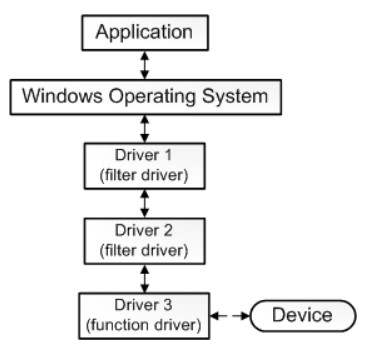
\includegraphics{images/Drivers.jpg}
				\caption{Request path through drivers\cite{MSDNWhatIsADriver}}
				\label{fig:drivers}
			\end{center}
		\end{figure}
		\paragraph{}
		I/O requests are sent to device drivers packaged in IRPs (I/O request packets). An IRP is a structure containing request's information. An important role pays the following field from the IRP structure\cite{MSDNIORequests}:
		\bigskip
		
			\centerline{\textcolor{blue}{struct} \textcolor{cyan}{\texttt{\_IO\_STACK\_LOCATION}} *\textcolor{cyan}{CurrentStackLocation}}
		
		\bigskip	
		\paragraph{}
		The Windows I/O system consists of several executive components that together manage hardware devices and provide interfaces to hardware devices for applications and the system\cite{WindowsInternals}. It is a packet driven system, with requests being usually backed by structures named IRPs. It is also possible that these requests to bypass the IRP-driven mechanism and go straight to the driver to complete the I/O request. This mechanism is called "Fast I/O".
		
		The I/O manager is responsible with IRP lifecycle management and also with passing them to the correct device stack in order to be properly processed. This places the I/O manager at the core of the I/O system. 
		
		
		The operating system abstracts all I/O requests as operations on a virtual file because the I/O manager has no knowledge of anything but files, therefore making it the responsibility of the driver to translate file oriented comments (open, close, read, write) into device-specific commands\cite{WindowsInternals}. As an example, a driver implementing pipe/FIFO mechanics would complete the read/write requests using the in-memory buffers instead of having an actual underlying physical device. 
		
		As it can be seen, the I/O system is very similar to the Linux VFS as it also provides a common interface that is implemented by both file system and pseudo-file system drivers (ProcFS - file system-like interface for querying process information).\\
		
	
		\begin{figure}[h!]
			\begin{center}
				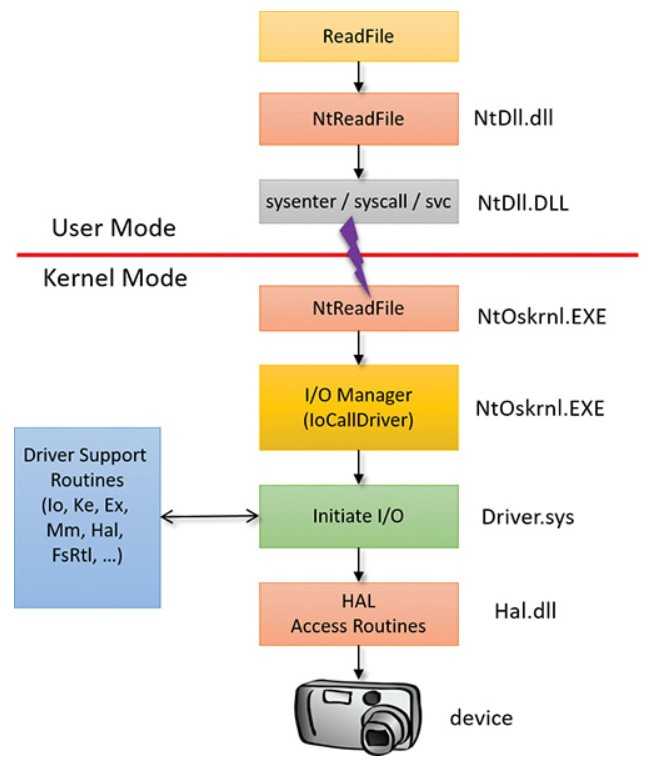
\includegraphics[scale=0.9]{images/IORequest.jpg}
				\caption{The flow of a typical I/O request\cite{WindowsInternals}}
				\label{fig:IORequest}
			\end{center}
		\end{figure}
		\pagebreak

		The common I/O processing path can be seen in image \ref{fig:IORequest}.

		Firstly, the application issues a system call to the operating system. Then, once it reaches the kernel, an IRP is allocated and sent to the corresponding driver. The driver can resolve the request by sending one or multiple I/O requests towards a physical device. It can also resolve the request without the help of any physical hardware support by considering the request to be for a virtual resource (i.e. filter port, pipe).
		
		
		\paragraph{}
		An IRP contains multiple useful pieces of information, like completion status, pend state, data buffer, etc. It also contains an array of IO\_STACK\_LOCATION structures which contain IRP parameters (i.e. creation flags, read/write buffer sizes). There is one stack location for each driver on the stack. When the IRP is passed down the stack, each driver is responsible with setting up the I/O stack location for the next driver in the stack either by copying the existing one or by setting up a completely different one. For example, an activity monitor would pass the parameters as they are to the next driver, but an encryption filter would change the parameters because it has to encrypt the data, thus leading to different buffer contents and buffer sizes.
		
		
		The I/O stack location of an IRP is comprised of the following information\cite{MSDNIOStackLocations}:
		\begin{itemize}
			\item IRP\_MJ\_*  - a major function code that the driver should handle
			\item IRP\_MN\_*  - a minor function code which indicates a particular case of a major operation. This can be found for example in PnP (Plug and Play) drivers. 
			\item A set of arguments related to the operation that should be performed, like the offset from where the driver starts reading and length that should be read.
			\item A pointer to the device object representing the target device for requested operation.
			\item A pointer to the file object which can be for example an open file or directory
		\end{itemize}
		
		\paragraph{}
		As some basic examples of major IRPs which are also common, the following can be considered:		
		\begin{itemize}
			\item \texttt{IRP\_MJ\_CREATE} - describes a request to open a handle to a resource
			\item \texttt{IRP\_MJ\_WRITE} - contains a buffer with data to be transferred to a device.
			\item \texttt{IRP\_MJ\_READ} - describes a buffer which the driver can fill in with data from a device.
			\item \texttt{IRP\_MJ\_CLEANUP} - this IRP is issued when all handles to a file object are closed.
		\end{itemize}
	
		\paragraph{}
	   	In order to get information regarding the I/O performed operation in a  driver \textcolor{blue}{IoGetCurrentIrpStackLocation} has to be called . After the desired operations have been performed in the current high-level driver, the developer   must set up the I/O stack location for the next driver\cite{MSDNIOStackLocations}.
	   
	   	\paragraph{}
	   	In terms of ways to organize a driver, there are multiple driver models such as Legacy Model, WDM (Windows Driver Model) or WDF (Windows Driver Foundation). The models consist of a set of API's that ease the development process. Depending on what type of driver a developer wants to implement a model can be chosen. In general, drivers can be of the following types: bus drivers, function drivers and filter drivers. 
	   	
	   	\paragraph{}
	   	A bus driver is responsible with individual I/O bus devices. Bus drivers are required and there usually exist bus drivers for every type of bus on the machine. This type of driver can also report child devices connected to the bus. Microsoft and OEMs usually offers a set of common bus drivers such as USB, PCI and many others\cite{MSDNWDMDrivers}.
	   	
	   	\paragraph{}
	   	Function drivers are the main driver for a device providing its operational interface. They usually handle writes, reads and manages device's power policy. This type of drivers can service more than one device\cite{MSDNWDMDrivers}.
	   
	   	\paragraph{}
	   	Finally, filter drivers are optional drivers which filter I/O requests thus making a change in device's usual behavior. Like functional drivers, a filter driver can service more than one device. Filter drivers can be of types: bus filter drivers, lower-level filter drivers and upper-level filter drivers\cite{MSDNWDMDrivers}.
	   
	   	\paragraph{}
	   	For a better understanding of filter drivers an example would be a driver that encrypts the disk data. It's functionality is to encrypt everything that goes to the disk and also decrypt the content requested from upper drivers. Therefore, the said filter driver could be an upper filter for the disk driver.
	   
	   	\paragraph{}
	   	From this example we can easily see that the way drivers are structured is in compliance with the first two SOLID principles. The single responsibility principle is backed up by the fact that every driver should handle one particular functionality that is easy to maintain with respect to other drivers. Also, the open-closed principle is followed because if Microsoft or a third party driver vendor wants to have a new functionality it can be written as a new filter driver to extend the functionality the old ones were offering. This way the old functionality is still provided, and the new ones can work independently without modifying the old components.
	   
	   	\paragraph{}
	   	Figure \ref{fig:driverstack} displays a driver stack containing basic drivers in a stack. The bus driver is at the bottom of the stack because it is closest to hardware. Filter drivers, which are optional, add functionality to the bus an function drivers. And finally, the function driver is the one which provides the operational interface for the device.
	    
	   	\begin{figure}[h!]
	   		\begin{center}
		   		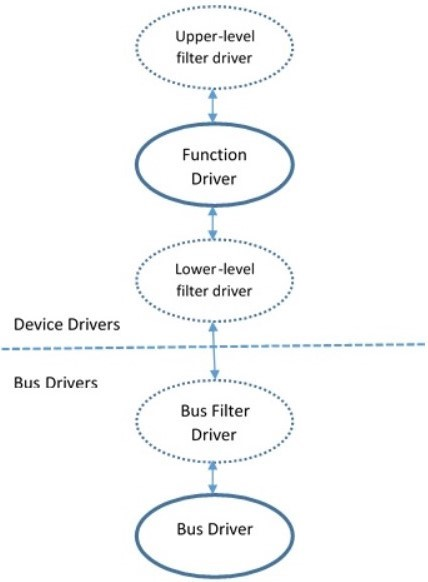
\includegraphics[scale=0.7]{images/DriverStack.jpg}
		   		\caption{Driver stack\cite{WindowsDriverTutorial}}
		   		\label{fig:driverstack}
	   		\end{center}
	   	\end{figure}
	   
	   
		\subsection{Windows Filter Manager}
		\paragraph{}
		During the years, a lot of problem with legacy filter drivers were starting to push the developer community to find solution to ease filters development. One great inconvenience is the fact that all IRP operation must be processed thus being a hard process. Due this and many other reasons, Microsoft decided to come with a solution regarding file system filters, which has been the development of Windows Filter Manager Driver. Nowadays files system filters are not supported anymore on newest Windows versions.
		
		\paragraph{}
		Filter Manager is a Windows driver containing functionality commonly required by drivers that intend to filter the file system. This set of functionalities is installed by default on Windows, but it only becomes active when a minifilter driver is loaded\cite{MSDNFltMgrConcepts}. Some of the features from Filter Manager are loading/unloading a minifilter any time, having more control over where the minifilter is loaded in terms of altitude and also volume it attaches to and the most important feature being the possibility to filter IRPs by registering callbacks that are called before the operation is started (Pre callbacks) and after the operation is completed (Post callbacks). 
		
		\paragraph{}	
		Pre callbacks can be used to provide additional functionality to the file system stack, allowing developers to complete the IRP themselves. Post callbacks are useful when a decision must be made based on the IRP completion information (i.e. status). Both pre and post callbacks have two important input parameters: \\ a PFLT\_CALLBACK\_DATA structure and a PCFLT\_RELATED\_OBJECTS structure. The first one is a view over the IRP that is presented to the minifilter driver. The second one is a structure that contains pointers to the objects that are related to the operation being processed (i.e. Volume, FileObject).
		
		\paragraph{}
		The altitude is a unique string identifier, interpreted as a number, which represents the position where a minifilter driver is loaded relative to other minifilters. The allocation of altitudes is managed by Microsoft thus the developers having to request an altitude in order to launch their driver into the market\cite{MSDNFltMgrConcepts}.
		
		\paragraph{}
		In minifilters, and not only, there are a set of load order groups for file system filters, which are loaded at system startup. These load order groups represent the order in which drivers will be loaded in memory\cite{MSDNFltMgrConcepts}. Load order groups are common for legacy filter drivers and minifilters, but the difference is that minifilters have the altitude therefore having an exact order in which the drivers will be loaded in spite of legacy filter drivers where filters having the same load order group will be loaded in memory in a random order.
		
		\begin{figure}[h!]
			\begin{center}
				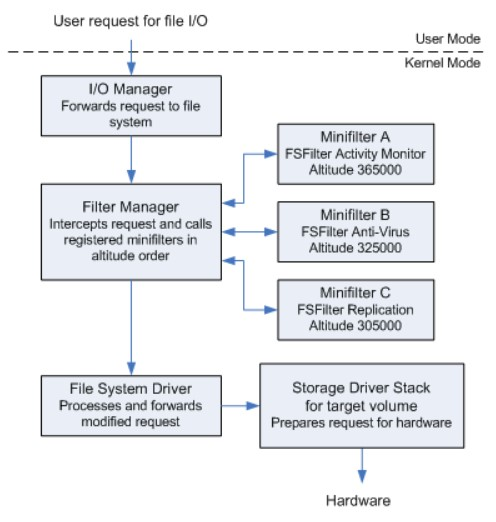
\includegraphics{images/FilterManager.jpg}
				\caption{Filter Manager \cite{MSDNFltMgrConcepts}}
				\label{fig:filterManager}
			\end{center}
		\end{figure}
		
		
		\paragraph{}
		In figure \ref{fig:filterManager} we can see the path an I/O request can take from User Mode through Kernel Mode. First of all, the user request transforms into an IRP initialized by the I/O manager. After creation, the IRP gets passed through drives, one of them being Filter Manager. Next step is to pass the IRP through every minifilter registered with Filter Manager until  last minifilter is reached or until completion. After the last minifilter is reached and the IRP has not been completed, the IRP goes through the next drivers until it reaches the lowest one in the stack.
		
		\paragraph{}
		Setting the I/O stack location is no longer a concern for the developer because Filter Manager has this functionality already implemented.
			
	\newpage		
	\section{Design and Implementation}
		\paragraph{}
		In this chapter I will start to explain in detail the main features of the developed application. Following steps are to explain the logic for file blocking which is the key feature of the application. Also, for a better understanding of the whole process I will present the communication between application's components. Finally, as the development process is not easy for a new developer, I will state some of the challenges which were encountered.
	
		\subsection{High Level Overview of Design}
		\paragraph{}
		Designed application is layered in 3 main components (fig.\ref{fig:FPMAinComponents}):
		\begin{itemize}
			\item fpf.sys
			\item FileProtectorCore.dll
			\item FileProtectorUI.exe
		\end{itemize}
		
		\paragraph{}
		The first component, fpf.sys, is a minifilter driver built in C. It encapsulates the logic for file blocking. The minifilter driver communicates with the dll through a filter port.
		
		\paragraph{}
		Secondly, FileProtectorCore.dll, built in C, exposes a set of APIs which can be used to communicate with the driver from a user mode application. This dll can be used for future integration in another applications.
		
		\begin{figure}[h!]
			\begin{center}
				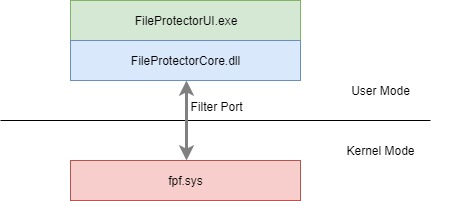
\includegraphics{images/fpMainComponents.jpg}
				\caption{File Protector main components}
				\label{fig:FPMAinComponents}
			\end{center}
		\end{figure}
		
		
		\paragraph{}
		Last component represents the GUI (fig \ref{fig:FPMainWindow}) that was developed with WPF which is part of .NET Framework. This application is always running and it can be found on the system tray. Users have the following features:
		
		\begin{itemize}
			\item adding a file to a protected files list
			\item removing a file from the protected files list
			\item start or stop file blocking
			\item see a history with allowed/denied files
			\item see statistics about protected files
		\end{itemize}
		
		\begin{figure}[h!]
			\begin{center}
				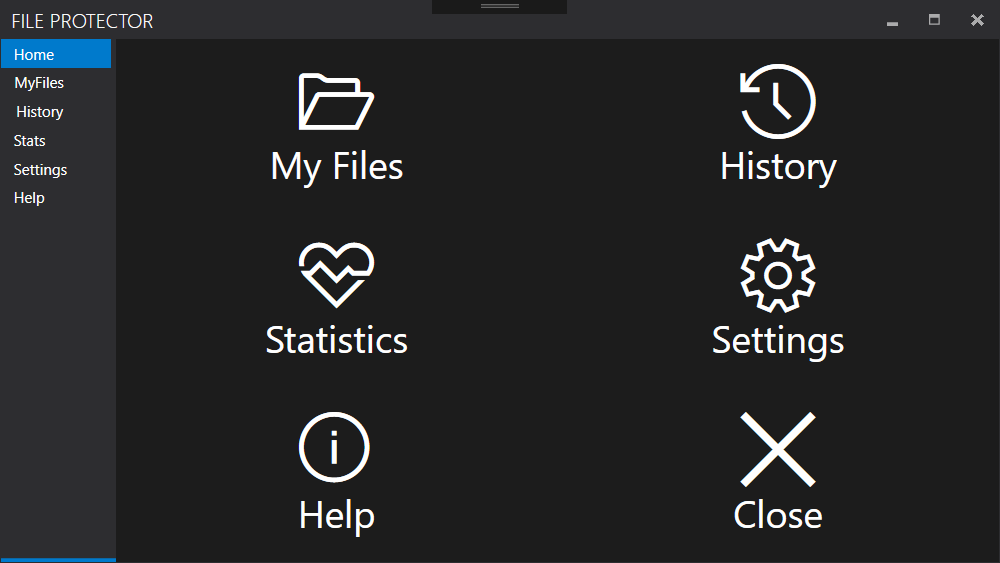
\includegraphics[scale=0.7]{images/FileProtectorMainInterface.PNG}
				\caption{File Protector main window}
				\label{fig:FPMainWindow}
			\end{center}
		\end{figure}
	
		Figure \ref{fig:FPMainWindow} represents the Home tab of the application. The first option, "My Files" displays a list with protected files and allows adding and removing files to the list. The History tab exposes a list of files that were accessed and whether they were allowed or not. There is also a tab of statistics where a graphic with allowed and denied files is displayed. Moreover, there is a settings tab where the user can turn the file blocking on or off and also an option which can be enabled in case user want to auto-block all incoming file open events. Finally, the help tab shows users information about the product.
		
		\newpage
		\subsection{Monitoring and Denying Access}
		\paragraph{}
		This subsection emphasizes the main feature of the application, the file blocking. This is accomplished using the Filter Manager framework by filtering IRP\_MJ \_CREATE IRPs issued down the file system stack and matching file paths against a database of known protected files. 
		
		
		This is achieved by registering pre and post callbacks by calling FltRegisterFilter. I/O operations filtering is started by calling FltStartFiltering. Denying access is achieved by completing the IRP\_MJ\_CREATE in the pre callback and also setting the IoStatus.Status field of the \textcolor{Emerald} {PFLT\_CALLBACK\_DATA} input parameter to \textcolor{Magenta} {STATUS\_ACCESS\_DENIED}.
		
		\begin{figure}[h!]
			\begin{center}
				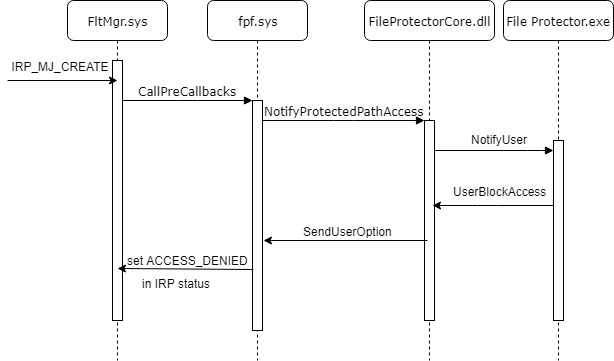
\includegraphics[scale=0.7]{images/SequenceDiagram.jpg}
				\caption{File Blocking}
				\label{fig:FPFBlockFileDiagram}
			\end{center}
		\end{figure}
	
		\paragraph{}
		Diagram \ref{fig:FPFBlockFileDiagram} shows a flow where a file from the protected files list is accessed and the user chooses to deny access to it. When a file is about to be opened, an IRP\_MJ\_CREATE is sent to the Filter Manager which calls the Pre callbacks for all registered minifilters with the \textcolor{Emerald} {PFLT\_CALLBACK\_DATA} structure containing a view of the IRP. fpf.sys has to get the file path by calling FltGetFileNameInformation. As parameters, this function requires the \textcolor{Emerald}{PFLT\_CALLBACK\_DATA}, \textcolor{Emerald} {FLT\_FILE\_NAME \_OPTIONS} which specifies the name format for the returned file path, and lastly \textcolor{Emerald} {PFLT\_FILE\_NAME\_INFORMATION} which is an output parameter where the file path will be stored. 
		
		\newpage
		The following code is the minifilter's call of FltGetFileNameInformation:
		
		\begin{Verbatim}[fontsize=\small, commandchars=\\\{\}]
		FltGetFileNameInformation(\\
		              \textcolor{Gray}{Data}, \\
		              \textcolor{magenta}{FLT\_FILE\_NAME\_NORMALIZED \textbar} \\
		              \textcolor{magenta}{FLT\_FILE\_NAME\_QUERY\_ALWAYS\_ALLOW\_CACHE\_LOOKUP}, \\
		              \&fileInformation \\
		)
		\end{Verbatim}
		
		\textcolor{magenta}{FLT\_FILE\_NAME\_NORMALIZED} is required to get the normalized name. The other possibility was using \textcolor{magenta}{FLT\_FILE\_NAME\_OPENED} but this could possibly give us unresolved paths (i.e. short paths), basically returning the path that was used to open the file. Short paths in Windows are created in case of file names longer than MS-DOS 8.3 naming convention, meaning the file name should have maximum 8 characters and it's extension maximum 3 characters.
		
		This is potentially dangerous because a malicious application could try to bypass the File Protector by accessing a file through its short name. Example of short for paths: c:\textbackslash test\textbackslash shortpathtest1.txt, c:\textbackslash test\textbackslash shortpathtest1.txtlong and \\ c:\textbackslash test\textbackslash shortpathtest1.txtlong \ref{fig:ShortPaths}
		
		\begin{figure}[h!]
			\begin{center}
				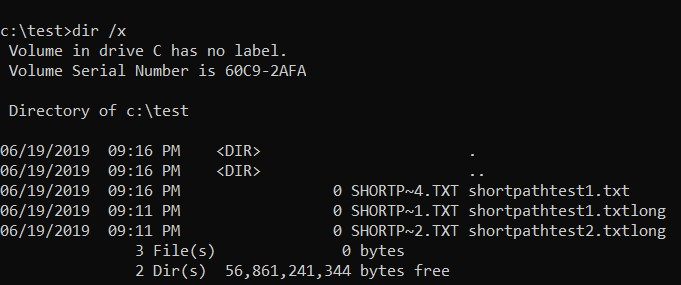
\includegraphics{images/ShortPaths.jpg}
				\caption{Short Paths}
				\label{fig:ShortPaths}
			\end{center}
		\end{figure}
	
		It can be seen how the filename is truncated and appended a tilde and an index (i.e. SHORTP~1\ref{fig:ShortPaths}). In order to obtain the "real" NT path, we need to normalize the path by using the flag previously described.
		
		\textcolor{magenta}{FLT\_FILE\_NAME\_QUERY\_ALWAYS\_ALLOW\_CACHE\_LOOKUP} first checks filter manager cache if name is already resolved. In case it is not, it queries the file system for the file name, by opening the file, if it is currently safe to do so.
		
		\paragraph{}
		After the path has been solved, a notification is sent into the dll using FltSendMessage. The communication needs a \textcolor{Emerald}{PFLT\_PORT} which needs to be created with FltCreateCommunicationPort in the minifilter and opened with FilterConnectCommunicationPort in the dll. Then the message is retrieved and a toast notification is displayed. \ref{fig:ToastNotification}
		
		\begin{figure}[h!]
			\begin{center}
				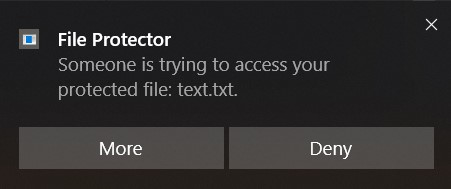
\includegraphics{images/ToastNotification.jpg}
				\caption{Toast Notification}
				\label{fig:ToastNotification}
			\end{center}
		\end{figure}
	
		\paragraph{}
		In case the "More" button is pressed, a secure desktop will be opened displaying the full path and the process trying to open the file. The secure desktop is necessary because we need to create a window that cannot get messages from any other process. By creating a new desktop specifically for our window, other processes will not be able to send messages (i.e. SendMessage, PostMessage) to our window because they will not have a handle for it. For a new desktop to be created, the following functions needed to be imported from user32.dll and kernel32.dll: GetThreadDesktop, GetCurrentThreadId, CreateDesktop, SwitchDesktop, SetThreadDesktop and CloseDesktop. 
		
		\paragraph{}
		Firstly, the old desktop should be preserved for recall and that was done by calling GetThreadDesktop(GetCurrentThreadId()) and keeping the returned value into a variable. To create the desktop and make it visible the calls should be performed in this order: CreateDesktop, SwitchDesktop. After the user made a choice, the old desktop must be restored to the initial state preforming the following calls: SwitchDesktop, SetThreadDesktop, CloseDesktop. 
		
		After the user denies the file opening, user's option is sent to the dll which sends it further to the minifilter by calling FilterSendMessage. The driver will block the file depending on users' response. 
	
	
		\subsection{Inter Component Communication}
		\paragraph{}
		As said before, communication between the minifilter driver and the dll are done through a filter port. The cases where the dll and the driver need to communicate are the following:
		\begin{itemize}
			\item when a user adds a file to the protected files list a notification must be sent from user mode to kernel mode
			\item when a file that is protected is opened the minifilter must send a notification to user mode for user approval
		\end{itemize}
			
		\paragraph{}
		Communication between user mode and kernel mode is supported by the Filter Manager. The minifilter driver can create a communication port which will begin to listen for incoming connections by default. 
		
		Port's security is handled in the minifilter driver by specifying a security descriptor. Among  Windows APIs we can find a variety of functions regarding creating and initializing a security descriptor for a new object from which I used FltBuildDefaultSecurityDescriptor. This function builds a security descriptor that can be further applied to a communication port which means only users with system administrator privileges will have access to the port\cite{MSDNCommunication}.
		
		\paragraph{}
		FltCreateCommunicationPort demands 3 callbacks used for communication between kernel mode and user mode: one that will be called when a client connects on the port, one that is called when a client disconnects, and one which is called when user mode applications call FilterSendMessage to send a message to the minifilter driver through the port\cite{MSDNCommunication}.
		

		For a client to connect on the filer port, FilterConnectCommunicationPort must be used. After the call has succeeded, FilterSendMessage can be used to communicate from user mode to kernel mode and FilterGetMessage is used to wait for messages sent from kernel mode to user mode\cite{MSDNCommunication}.
		
		
		\paragraph{}
		The path of a file can contain multiple components separated by a backslash. The prefix of a path, which determines the namespace, depends on system's interpretation. In user mode, full file paths start with a drive letter (volume name) followed by a backslash like C:$\backslash$ or D:$\backslash$. Another way of naming files is using the Universal Naming Convention (UNC), which is commonly used for accessing remote file shares (i.e. $\backslash$$\backslash$ServerName$\backslash$ShareName$\backslash$FileName).
		
		\begin{figure}[h!]
			\begin{center}
				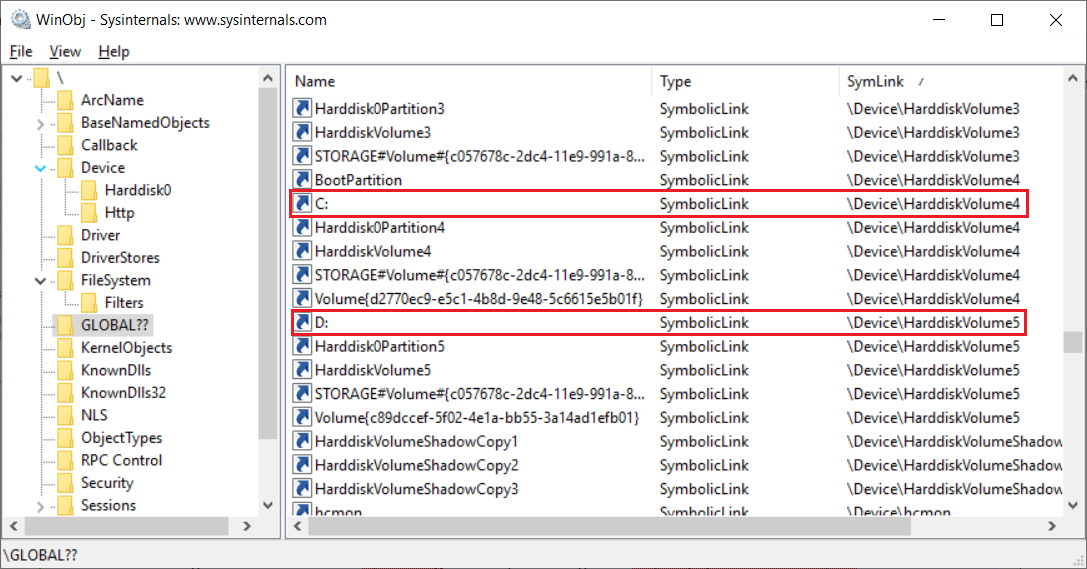
\includegraphics[scale=0.6]{images/WinObj.jpg}
				\caption{WinObj GLOBAL?? namespace}
				\label{fig:WinObj}
			\end{center}
		\end{figure}
		
		The Windows kernel uses NT paths, meaning that volumes will be named differently from the usual user mode volume name, like "$\backslash$Device$\backslash$HarddiskVolume4" instead of the C:$\backslash$ drive letter. For example, if we have the DOS path C:$\backslash$folder1$\backslash$file.txt, the corresponding NT path will be similar to: $\backslash$Device$\backslash$HarddiskVolume4$\backslash$folder1$\backslash$ file.txt  \cite{MSDNNamespaces}. That's because "C:" is a DOS device, which is actually a symbolic link to the actual device (i.e. $\backslash$Device$\backslash$HarddiskVolume4).
		
		WinObj is a Windows Sysinternals tool that uses Windows APIs to access and display information about namespaces. If we go to the GLOBAL?? namespace in WinObj, we can see that C: and D: have as symbolic links $\backslash$Device$\backslash$ HarddiskVolume4 and $\backslash$Device$\backslash$HarddiskVolume5, as highlighted in figure figure \ref{fig:WinObj} .
		
		When paths are sent from user mode to kernel mode, they must be converted to NT paths by resolving the drive letter symbolic link by calling the ZwQuerySymbolicLinkObject API.
		
		\subsection{Encountered Challenges}
		\paragraph{}
		 A minifilter driver development process is different from what most of programmers are used to because it requires a lot of attention and especially knowledge of Windows drivers in order to get a satisfying end result.
		
		\paragraph{}
		One of the first challenges I want to talk about is testing. Windows drivers must be tested on a test machine, because any little mistake could lead to compromising system's availability. In order to test my code I've created a Windows 10 Pro x64 virtual machine. For drivers to be loaded, Windows requests drivers to be signed with a Microsoft certificate. However, for testing purposes the drivers can be signed with a test certificate and thus Windows does not load test-signed drivers. 
		
		\paragraph{}
		In order to load a driver with a test signature the machine has to be set to test mode which is done through following commandline (it must be opened with administrator rights):
		
		\bigskip
		\centerline {\texttt{bcdedit -set testsigning on}}
		\bigskip
		
		\paragraph{}
		The result can be seen almost immediately because a watermark will be shown on the lower right side of the screen and the driver with test signature can be loaded.
		
		\paragraph{}
		Another challenge was debugging the driver. Because every bug would lead to a BSOD, debugging is a good solution when it comes to testing newly added code. Similar to setting the machine as a test one, kernel debugging should be enabled with the command:
		
		\bigskip
		\centerline {\texttt{bcdedit -set debug on}}
		\bigskip
		
		\paragraph{}
		 When it comes to creating a new desktop, WPF does not support creating windows in the newly created desktop. A solution for this issue was creating a Windows Forms Window instead of a WPF one, and it will be displayed correctly.
		
	\newpage
	\section{Testing Approach}
		\paragraph{}
		In order to achieve a reliable software, the application has been tested using both black box and white box (i.e. static code analysis) testing methods, which will be described in the following sections.
		
		\subsection{Driver Verifier}
		\paragraph{}
		The "Driver Verifier" monitors drivers in order to detect illegal function calls or actions that might corrupt the system\cite{MSDNDriverVerifier}. Examples of such actions are:
		\begin{itemize}
			\item memory leaks
			\item memory corruptions such as buffer overflows or underflows
			\item deadlocks
		\end{itemize}
	
		 It is highly configurable, allowing the developer to enable individual checks for individual drivers.
		
		\begin{figure}[h!]
			\begin{center}
				\includegraphics[scale=0.8]{images/DriverVerifier.png}
				\caption{Driver Verifier Options}
				\label{fig:DriverVerifierOptions}
			\end{center}
		\end{figure}
		
		\newpage
		Some of the features that were used in testing the File Protector are:
		\begin{itemize}
			\item special pool - for detecting memory corruptions
			\item pool tracking - checks for memory leaks
			\item security checks - monitors common mistakes that result in security issues
			\item systematic low resource simulation - inserts artificial API failures in order to verify that the driver treats fail cases accordingly
		\end{itemize}
		
		\subsection{Static Code Analysis}
		\paragraph{}
		In this section I will talk about source code annotation language (SAL). This is used to make the code more explicit, in terms of behavior, parameters or return values to make it more understandable. In other words, programmer's work is to use annotations considering the desired functionalities, and compiler's work is to verify if the written code corresponds with the annotations. 
		
		\paragraph{}
		All SAL annotations have a specific "look", and that is \texttt{\_Annotation\_name\_}. For example, some parameter most used SAL annotations are \textcolor{magenta}{\texttt{\_In\_}} and \textcolor{magenta}{\texttt{\_Out\_}}. \textcolor{magenta}{\texttt{\_In\_}} makes sure the compiler interprets data as being input data that cannot be modified in function's scope. \textcolor{magenta}{\texttt{\_Out\_}} allows the programmer to use the parameter as an output one, as long as the space for that parameter has been allocated by the programmer.
		
		\paragraph{}
		As for behavior, a simple example is \textcolor{magenta}{\texttt{\_Check\_return\_}}. If this annotation is used, the caller must inspect the returned value. In case the function has a void return type, an error will be shown at compilation time. A similar example is \textcolor{magenta}{\texttt{\_Must\_inspect\_result\_}}, which contains the functionality of \textcolor{magenta}{\texttt{\_Check\_return\_}} and adds that any output parameter should also be used after the function call.
		
		The following example is the MessageNotifyCallback that is called whenever a user calls FilterSendMessage to send a message to the driver. 
		
		\begin{Verbatim}[fontsize=\small, commandchars=\\\{\}]
\textcolor{Emerald}{NTSTATUS}
\textcolor{magenta}{FLTAPI} FpOnClientNotify(
\textcolor{magenta}{\_In\_opt\_} \textcolor{Emerald}{PVOID} \textcolor{Gray}{PortCookie},
\textcolor{magenta}{\_In\_reads\_bytes\_opt\_}(\textcolor{Gray}{InputBufferLength}) \textcolor{Emerald}{PVOID} \textcolor{Gray}{InputBuffer},
\textcolor{magenta}{\_In\_} \textcolor{Emerald}{ULONG} \textcolor{Gray}{InputBufferLength},
\textcolor{magenta}{\_Out\_writes\_bytes\_to\_opt\_}(\textcolor{Gray}{OutputBufferLength}, *\textcolor{Gray}{ReturnOutputBufferLength})
\textcolor{Emerald}{PVOID} \textcolor{Gray}{OutputBuffer},
\textcolor{magenta}{\_In\_} \textcolor{Emerald}{ULONG} \textcolor{Gray}{OutputBufferLength},
\textcolor{magenta}{\_Out\_} \textcolor{Emerald}{PULONG} \textcolor{Gray}{ReturnOutputBufferLength}
)
		
		\end{Verbatim}
		
		\newpage 
		\paragraph{}
		The SAL annotations encountered here have the following meanings:
		\begin{itemize}
			\item \textcolor{magenta}{\_In\_} - input parameters are treated as read-only 
			\item \textcolor{magenta}{\_In\_opt\_} - is used to indicate that there is an input parameter that may be also null.
			\item \textcolor{magenta}{\_In\_reads\_bytes\_opt\_}(s) - this means the function has to read from the array with size s that was given. The \_bytes\_ means that the size given is in bytes, not in elements. \_opt\_ allows also null values to be provided.
			\item \textcolor{magenta}{\_Out\_} - the caller of the function provides space for the output parameter, which the function must write to.
			\item \textcolor{magenta}{\_Out\_writes\_bytes\_to\_opt\_}(s, c) - here s represents the maximum size of an array in elements (bytes in this case), and c is the number of elements that must be valid in post-state. In this case, the output buffer can hold a maximum number of \texttt{OutputBufferLength} bytes, and \texttt{*ReturnOutputBufferLength} will hold the number of bytes that was actually written.
		\end{itemize}
		
		\paragraph{}
		This mentioned examples emphasize why SAL is beneficial, and that is also why it was used for the minifilter driver development.
	